\chapter{循环神经网络加速技术基础}

\section{循环神经网络及其变体}
循环神经网络是一种专门针对序列数据进行建模的神经网络模型。有别于前馈神经网络,卷积神经网络等“静态模型”,循环神经网络在结构上拥有循环
自连接的反馈机制,这使得模型当前的输出不仅取决于当前输入,还与当前的状态有关。通过对状态的存储与更新,循环神经网络能够有效的建模动态系统。
理论上,任何图灵可计算的函数都可以用有限维的循环网络近似。尽管循环神经网络功能强大,但是高昂的训练成本阻碍了循环神经网络的实际应用。
一方面,固定有序的前向传播过程只能遵循序列顺序先后计算,因此通过时间的反向传播无法并行计算;另一方面,梯度消失和梯度爆炸问题在循环神经网络
的训练过程中尤为突出,这导致其学习长期依赖关系变的困难。随着理论研究的发展和算力的提升,以上问题都得以解决。借助第三次人工智能浪潮
循环神经网络重新焕发出勃勃生机,目前,循环神经网络已经广泛应用于自然语言处理等相关领域。

\subsection{普通循环神经网络}
普通循环神经网络是最简单的循环神经网络结构,主要包括输入层,隐藏层和输出层。输入层对输入进行特征提取并映射为固定长度的向量,隐藏层将输入信息
和前一时刻的状态转化为新的状态,输出层根据网络存储的状态解码并完成输出。其中隐藏层包含记忆信息以及记忆更新的规则,是循环神经网络中最重要的
结构。
常见的循环神经网络结构如图\ref{fig:rnn}所示,权重矩阵\(U, W, V\)分别表示输入到到隐藏,隐藏到隐藏,隐藏到输出之间的连接,向量\(x, h, o\)分别表示输入单元,
隐藏单元和输出单元,这些单元及其相互连接形成网络。相比于其他网络模型的单向信息传递,循环神经网络引入环状结构实现了从输入到输出的双向信息
流动。一些符合训练准则的信息将会通过循环的方式长期保存在网络状态中,并根据输入序列特征进行适时唤醒记忆。当网络记忆的信息足够丰富时,循环神经
网络不仅能准确的预测输出,并且能大致恢复输入序列。自编码器框架就是基于此原理而产生,其能根据记忆的状态信息选择重要的输入并近似复制到输出,
实现特征学习或降维。图中左侧为循环神经网络回路原理图,黑色方块表示回路中单个时间步的延迟,即时刻t-1的状态会影响时刻t的状态。图中右侧为
循环神经网络按时间展开的计算图,展开是指将左侧的回路结构映射为右侧的包含重复组件的结构,展开的深度取决与序列的长度。循环神经网络展开结构图
显式的数据流动路径描述了信息是如何在时间上向前和向后传递的。
\begin{figure}
	\centering
	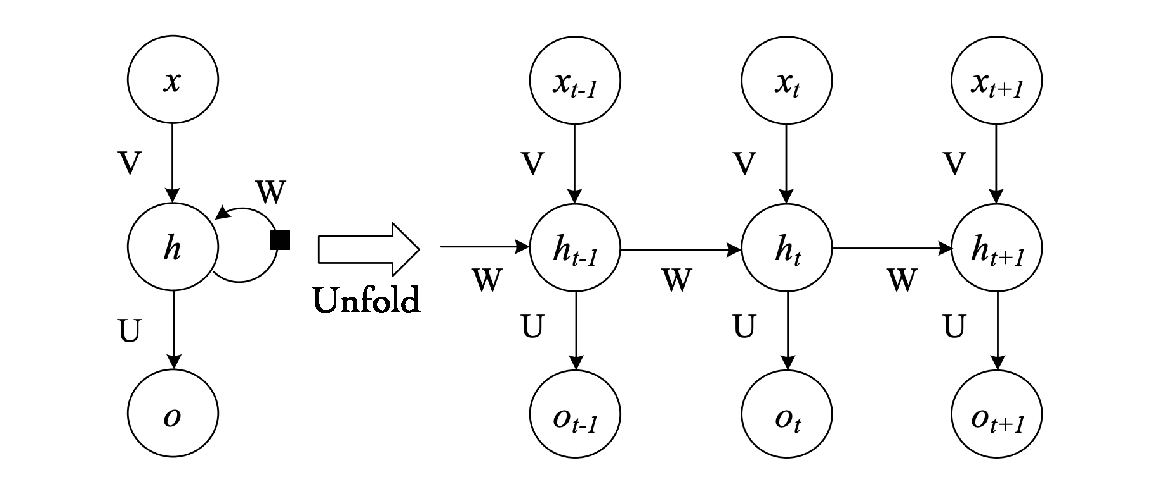
\includegraphics[width=0.8\columnwidth]{RNN_struct.eps}
	\caption{普通循化神经网络结构图}
	\label{fig:rnn}
\end{figure}

循环神经网络的数学模型为式\ref{eq:rnn}, 其中\(g\), \(f\)分别表示隐藏层和输出层的激活函数。在循环神经网络中\(g\)一般选用\(sigmoid\),\(tanh\)
等饱和性激活函数以避免训练过程中可能出现的梯度爆炸问题。函数表达式除了描述模型输入与输出的关系外,还规定了循环神经网络内部结构的
一般特性:

(1)状态的长度固定,即模型的记忆容量有限。\(h_t\)作为过去序列与任务相关方面的有损摘要,只能根据训练准则选择性的保留过去序列的某些方面特质。

(2)模型单个时间步的输入是固定的。无论序列的长度,模型每个时刻始终具有相同大小的输入,状态转移也只能从一种状态转移到下一种状态,
而不是在可变长度的输入序列或历史状态上进行操作。

(3)每个时间步使用相同参数的相同转移函数,即输出的每一项是对先前输出应用相同的更新规则而产生的。更新规则在时间上共享,模型能够表示序列间的相互影响。
相比在所有时间步均建立独立的学习模型,单一的共享模型在非训练集的序列上具有良好的泛化能力。

\begin{equation}\label{eq:rnn}
	\begin{split}
		h_{t} &= g(W*h_{t-1} + U*x_{t})	\\
		y_{t} &= f(V*h_{t})						
	\end{split}
\end{equation}

循环神经网络的训练采用通过时间的反向传播算法(Back-propagation through time,BPTT)。梯度计算首先将一段序列依次送入模型进行前向传播,
保存前向传播过程中的各个状态并计算最终的损失函数;然后,计算梯度并沿时间反向更新权重参数。由于循环网络的计算涉及相同函数的多次组合,
无论沿时间正向或者反向,当需要捕获的依赖关系需要跨越很长的时间尺度时,输入和输出会出现极端的非线性行为。具体的,如果雅可比矩阵的最大特征值
小于1,多次连乘后梯度会趋于0,梯度消失会使得模型参数无法更新,梯度下降算法永远不会收敛到最优解;如果雅可比矩阵的最大特征值大于1,那么随着
时间跨度的增大,梯度也将越来越大,最终会导致权重剧烈改变,学习也变得不稳定。梯度消失和梯度爆炸问题使得循环神经网络学习序列的长期依赖
关系变得困难, 目前,研究人员提出了一些降低学习长期依赖难度的方法,在某些情况下循环神经网络可以学习跨越百步的依赖关系,尽管取得了很大的进步
但是,如何学习更长时间的依赖关系仍然是深度学习领域的一个主要挑战。


\subsection{长短期记忆神经网络}
长短期记忆神经网络(Long short-term memory,LSTM)是目前应用范围最广的一种循环神经网络,相比简单的循环架构,LSTM能更容易的学习到长期依赖。
其结构中存在多层循环,除了外部的循环外,内部还存在“LSTM细胞”自循环。多层循环使得时间路径增加,梯度消失的可能性被大大降低,因此更深的循环神经
网络架构也得以实现\citing{}。

LSTM网络结构如图\ref{fig:lstm}所示,输入信息需要经过多条数据路径并进行复杂的加工处理才能最终到达隐藏层,这些位于数据路径中的“门”控制着信息的通过率。
其值越接近1表示该信息越需要被记忆,越接近0表示信息应该迅速被丢弃。通过控制信息的通过率,网络能够在较长的时间内持续积累线索,并且尽量少的受
干扰信息影响,因此累积的时间尺度可以动态的调节。LSTM网络中的门主要包括输入门\(i\),遗忘门\(f\)和和输出门\(o\),网络的输入信息包括细胞态\(c_{t-1}\),
状态\(h_{t-1}\)以及输入\(x_t\)。

在LSTM网络的前向传播过程中,首先当前的输入\(x_t\)和上一时刻的状态\(h_{t-1}\)会共同生成遗忘门的通过率,上一时刻的细胞态\(c_{t-1}\)会在此门
的控制下选择性的通过。然后,在输入门的控制下,输入信息中的重要线索会被合并到新的细胞状态中。最后细胞当前的状态会通过输出门进行最终的
筛选并产生新的状态。以上输入信息和记忆信息在三个门控单元的层层作用下,序列中符合学习经验的信息将会在很长的时间尺度内被收集起来,实现长期记忆,
而无关的信息所形成的短期记忆则会随着时间流逝迅速被遗忘。图中上半部分LSTM网络的循环图,图中清晰的展示了细胞态和状态的时间回路;图中下半部分为
LSTM网络的展开图,同一组件按时间顺序依次排开形成时间维度的信息流动路径,图中不仅描述了单个时间步信息如何被处理,还描述了相邻时间步之间数据如何
被衔接。

\begin{figure}
	\centering
	\includegraphics[width=1\columnwidth]{LSTM_struct.eps}
	\caption{LSTM结构图}
	\label{fig:lstm}
\end{figure}

LSTM网络的数学模型为式\ref{eq:lstm},该表达式详细说明了LSTM网络从t=1到t=T的计算流程。其中\(W\)表示权重矩阵,\(b\)表示偏置向量,\(\odot\)运算符
表示向量按位相乘,\(+\)运算符表示向量按位相加,符号\(i\),\(f\),\(o\),\(c\)分别表示输入门,遗忘门,输出门和细胞状态。向量的按位乘法实际上表示
信息在门控单元的筛选下选择性的通过,门控单元的通过率不是固定不变的,而是根据上下文进行动态的调节。向量加法实际上可理解位信息合并的过程,
多条信息通路汇聚后信息通过简单的加和操作完成了信息的整合。

\begin{equation}\label{eq:lstm}
	\begin{split}
		&i_t = \sigma(W_{ix}*x_t + W_{ih}*h_{t-1} + b_i)	\\
		&f_t = \sigma(W_{fx}*x_t + W_{fh}*h_{t-1} + b_f)	\\
		&g_t = \tanh(W_{cx}*x_t + W_{ch}*h_{t-1} + b_c)					\\
		&c_t = f_t \odot c_{t-1} + g_t \odot i_t							\\	
		&o_t = \sigma(W_{ox}*x_{t} + W_{oh} * h_{t-1} + b_o)	\\
		&h_t = o_t \odot \tanh(c_{t})											\\												
	\end{split}
\end{equation}


\subsection{回声状态网络}
回声状态网络(Echo state network,ESN)是一种基于储层计算(reservoir computing)的神经网络,它通过固定循环矩阵巧妙的避免了循环神经网络
训练过程中梯度消失和梯度爆炸的问题,广泛应用于序列预测和动态系统建模。由于其易于训练,基于回声状态网络搭建的深度循环神经网络能够实现并应用,
这显著的增强循环神经网络学习和预测能力。此外,相比于其他循环神经网络,ESN结构更加简单,物理意义也易于解释。因此本文以回声状态网络为例,
提出并设计针对循环神经网络前向传播过程的加速系统,并将该系统基于FPGA硬件实现。

回声状态网络结构如图\ref{fig:esn}所示,其由输入层\(u\),隐藏层\(x\)(储备层)和输出层\(y\)组成。输入层将输入投影到高维的状态空间,信息的特征被
充分的提取并且变得线性可分。隐藏层由大量的神经元组成,数量通常达到几百或上千,这在其他种类的循环神经网络中几乎不可能实现。数量庞大的神经元
通过“回声”完成对输入序列动态特性的记忆,但是记忆的能力并不是来自于学习训练数据中的经验,而是自然形成。回声状态网络中的输入连接权重\(W_{in}\)
和隐藏层的自循环权重\(W\)在初始化阶段随机生成,在训练过程中始终保持固定不变,因此这两部分连接权重不能通过学习来获得。模型的记忆能力与
求解问题无关,这极大的降低了学习的成本。输出层的连接权重是ESN网络中唯一可以学习的参数,通过选择与任务高度相关的记忆及其变换方式,模型
可以满足特定系统的动力学要求。

回声状态网络的基本数学模型为式\ref{eq:esn},其中\(x\in \mathbb{R}^n\)表示隐藏层神经元数量为n,\(u \in \mathbb{R}^{n_{in}}\)和\(y \in \mathbb{R}^{n_{out}}\)
分别表示模型的单个时间步的输入为\(n_{in}\)维,输出为\(n_{out}\)维;权重矩阵\(W_{in} \in \mathbb{R}^{n \times n_{in}}\),\(W\ \in \mathbb{R}^{n \times n}\)和\(W_{out} \in \mathbb{R}^{n_{out} \times n}\)
分别表示输入层到隐藏层,隐藏层到隐藏层,隐藏层到输出层神经元之间的相互连接。\(W_{in}\)和\(W\)随机生成,不可训练。为解决系统的稳定性问题
需要设定\(W\)的谱半径\(SR < 1\)。为保证网络能够记忆足够的动态特性,隐藏层通常拥有大量神经元来超额记忆任务所需要记住的数据。

网络能力,计算量,可压缩量。


dd

dd

dd

\begin{figure}
	\centering
	\includegraphics[width=0.7\columnwidth]{ESN_struct.eps}
	\caption{ESN结构图}
	\label{fig:esn}
\end{figure}


\begin{equation}\label{eq:esn}
	\begin{split}
		x_{t} &= f(W*x_{t-1} + W_{in}*u_{t})	\\
		y_{t} &= W_{out}*x_{t})						
	\end{split}
\end{equation}




\section{模型压缩与加速算法}


\subsection{轻量化网络}

\subsection{模型稀疏化}

\subsection{数值量化}

\subsection{张量分解}

\section{硬件加速平台介绍}

\subsection{FPGA硬件加速技术}

\subsection{开发工具}


如图\ref{picb}和图\ref{picc}所示分别给出了参数$E_0=\hat{x}$,$a_n=-\hat{z}$,$f_0=250MHz$,$f_w=50MHz$,$t_w=4.2\sigma$时,调制高斯脉冲的时域与频域归一化波形图。

\begin{figure}[h]
\subfloat[]{
	\label{picb}
	\includegraphics[width=7.3cm]{picb.pdf}
}
\subfloat[]{
	\label{picc}
	\includegraphics[width=6.41cm]{picc.pdf}
}
\caption{调制高斯脉冲时域与频率波形,时域阻抗元素的存储技术也是时间步进算法并行化的关键技术之一。(a)调制高斯脉冲信号的时域波形;(b)调制高斯脉冲信号的频域波形}
\label{fig1}
\end{figure}

时域阻抗元素的存储技术\citing{xiao2012yi}也是时间步进算法并行化的关键技术之一,采用合适的阻抗元素存储方式可以很大的提高并行时间步进算法的计算效率。

\section{本章小结}
本章首先从时域麦克斯韦方程组出发推导得到了时域电场、磁场以及混合场积分方程。

